\documentclass[12pt,a4paper]{article}
\usepackage[utf8]{inputenc}
\usepackage{graphicx}
\usepackage{float}
\usepackage{amsmath}
\usepackage{enumitem}
\usepackage{booktabs}
\usepackage{hyperref}
\usepackage{listings}
\usepackage{xcolor}
\usepackage{geometry}

% Make sure LaTeX can find your images
\graphicspath{{./}}

\geometry{margin=1in}

\title{Multi-Core Cache Simulation Report}
\author{} % Add your name if needed
\date{\today}

\begin{document}

\maketitle
\tableofcontents
\newpage

\section{Simulation Structure and Implementation}

\subsection{Flowcharts}

\begin{figure}[H]
    \centering
    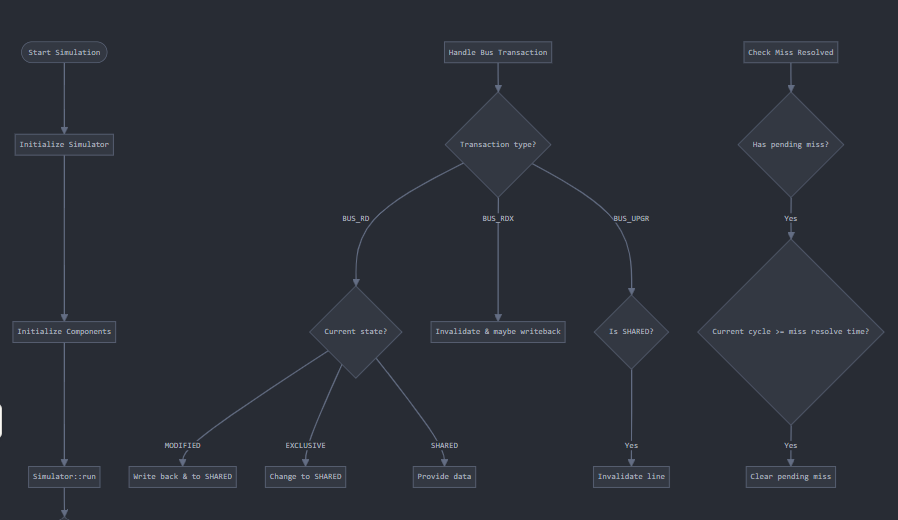
\includegraphics[width=0.9\textwidth]{image1.png}
    \caption{Flowchart depicting initialisation logic}
    \label{fig:init-logic}
\end{figure}

\begin{figure}[H]
    \centering
    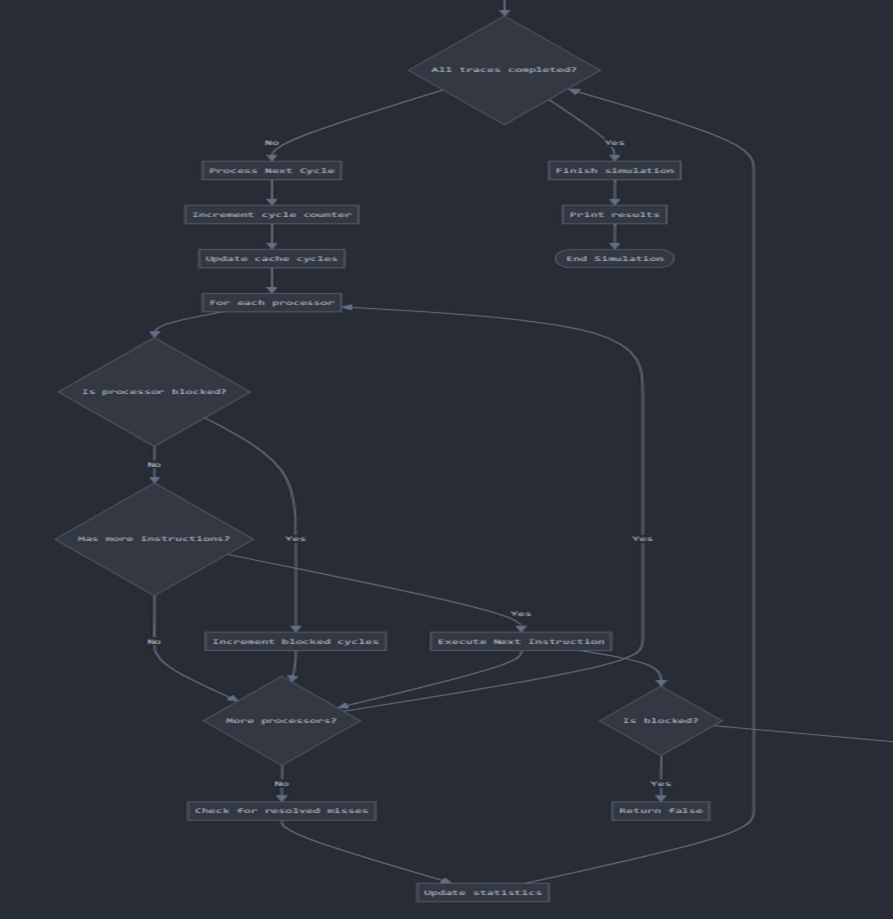
\includegraphics[width=0.9\textwidth]{image2.png}
    \caption{Flowchart depicting main loop logic}
    \label{fig:main-loop}
\end{figure}

\begin{figure}[H]
    \centering
    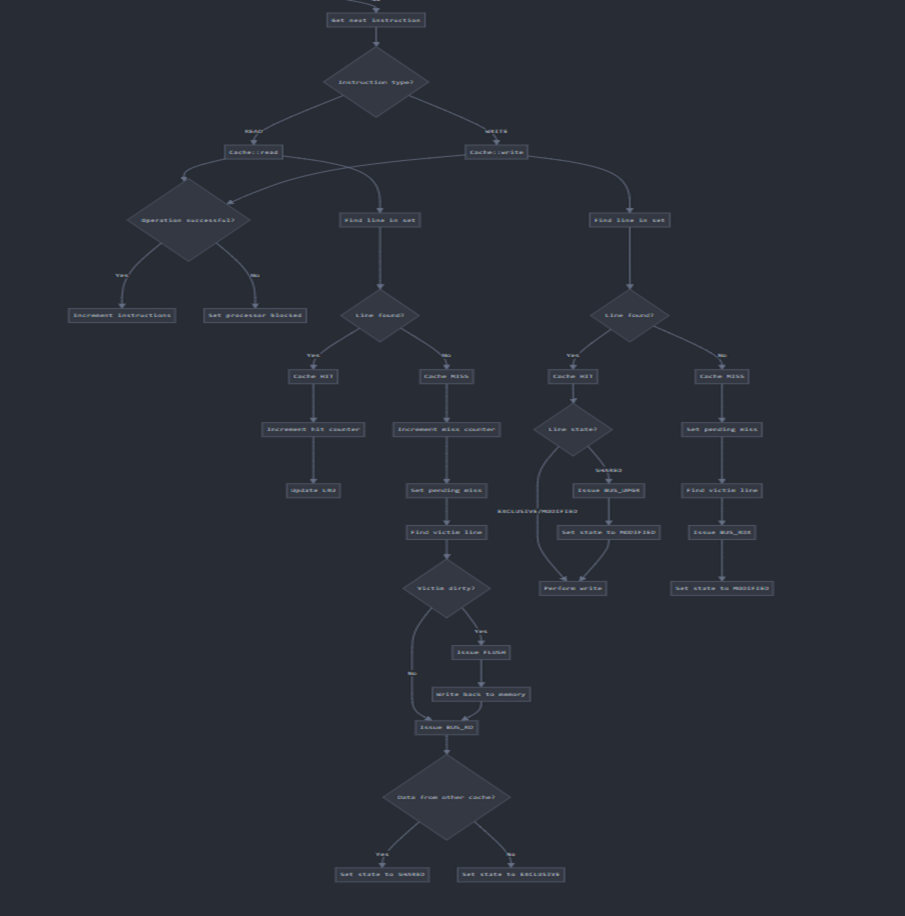
\includegraphics[width=0.7\textwidth]{image3.png}
    \caption{Still part of main loop; logic for blocks}
    \label{fig:block-logic}
\end{figure}

\subsection{Explanation of Classes and Functions}

\subsubsection*{File: Simulator.h / Simulator.cpp}

\textbf{Class: Simulator}

Main orchestrator for the entire multi-core simulation.

\textbf{Data Members:}
\begin{itemize}
    \item SimulationConfig config: Configuration parameters
    \item TraceReader traceReader: Reads instruction traces
    \item MainMemory mainMemory: Shared memory system
    \item std::vector<std::unique\_ptr<Cache>> caches: L1 caches (one per core)
    \item std::vector<std::unique\_ptr<Processor>> processors: CPU cores
    \item std::ofstream logFile: Output log file
    \item unsigned int currentCycle: Current simulation cycle
    \item Various statistics counters (instructions, cycles, hits, misses, etc.)
\end{itemize}

\textbf{Functions:}
\begin{itemize}
    \item Simulator(const SimulationConfig\& config): Constructor, initializes simulation
    \item \~{}Simulator(): Destructor, closes log file
    \item bool initialize(): Opens trace files and initializes components
    \item void initializeComponents(): Sets up caches, processors, and coherence callbacks
    \item void run(): Main simulation loop
    \item bool processNextCycle(): Advances simulation by one cycle
    \item void logStatistics(): Logs current statistics
    \item unsigned int getTotalInstructions() const: Returns instruction count
    \item unsigned int getTotalCycles() const: Returns cycle count
    \item double getAverageMemoryAccessTime() const: Calculates average memory access time
    \item unsigned int getInvalidationCount() const: Returns total invalidations
    \item unsigned int getBusTrafficBytes() const: Returns total bus traffic
    \item void printResults() const: Outputs simulation results to console
\end{itemize}

\subsubsection*{File: Cache.h / Cache.cpp}

\textbf{Class: Cache}

Implements an L1 cache with MESI coherence protocol.

\textbf{Data Members:}
\begin{itemize}
    \item int coreId: Core ID this cache belongs to
    \item MainMemory\& mainMemory: Reference to main memory
    \item int setBits, int blockBits: Address mapping configuration
    \item int numSets, int blockSize, int associativity: Cache configuration
    \item std::vector<CacheSet> sets: Cache sets
    \item CoherenceCallback coherenceCallback: Function for issuing coherence requests
    \item Various counters (access, hit, miss, read, write, coherence)
    \item bool pendingMiss: Flag for tracking unresolved misses
    \item unsigned int missResolveTime: Cycle when miss will resolve
    \item unsigned int currentCycle: Current simulation cycle
    \item int dataSourceCache: ID of cache that provided data on a miss
\end{itemize}

\textbf{Functions:}
\begin{itemize}
    \item Cache(int coreId, int numSets, int associativity, int blockSize, int setBits, int blockBits, MainMemory\& mainMemory): Constructor
    \item bool read(const Address\& addr): Handles read requests
    \item bool write(const Address\& addr): Handles write requests
    \item bool checkMissResolved(): Checks if a pending miss has been resolved
    \item void setCycle(unsigned int cycle): Sets the current cycle
    \item void setCoherenceCallback(const CoherenceCallback\& cb): Sets coherence callback
    \item void issueCoherenceRequest(...): Issues a bus transaction
    \item std::vector<uint8\_t> fetchBlockFromMemoryOrCache(...): Fetches a block
    \item bool handleBusTransaction(...): Processes bus transactions from other caches
    \item Various getters for statistics and configuration parameters
    \item const std::vector<CacheSet>\& getSets() const: Access to cache sets
    \item bool hasPendingMiss() const: Returns if there's a pending miss
    \item unsigned int getEvictionCount() const: Returns eviction count
    \item unsigned int getWritebackCount() const: Returns writeback count
\end{itemize}

\subsubsection*{File: Processor.h / Processor.cpp (Provided in the question)}

\textbf{Class: Processor}

Simulates a CPU core executing instructions.

\textbf{Data Members:}
\begin{itemize}
    \item int coreId: Core ID
    \item TraceReader\& traceReader: Reference to trace reader
    \item Cache\& l1Cache: Reference to this core's L1 cache
    \item bool blocked: Whether processor is blocked on a cache miss
    \item unsigned int cyclesBlocked: Number of cycles spent blocked
    \item unsigned int instructionsExecuted: Number of instructions completed
\end{itemize}

\textbf{Functions:}
\begin{itemize}
    \item Processor(int id, TraceReader\& reader, Cache\& cache): Constructor
    \item bool executeNextInstruction(): Attempts to execute the next instruction
    \item bool isBlocked() const: Returns if processor is blocked
    \item void setBlocked(bool state): Sets blocked state
    \item int getCoreId() const: Returns core ID
    \item bool hasMoreInstructions() const: Checks if there are more instructions
    \item unsigned int getCyclesBlocked() const: Returns cycles spent blocked
    \item unsigned int getInstructionsExecuted() const: Returns instructions executed
    \item void resetStats(): Resets processor statistics
    \item void incrementCyclesBlocked(): Increments blocked cycles counter
\end{itemize}

\subsubsection*{Other Important Classes (Referenced but not fully shown)}

\textbf{Class: CacheSet}

Represents a set of cache lines.

\textbf{Functions:}
\begin{itemize}
    \item CacheLine* findLine(uint32\_t tag): Finds a line with matching tag
    \item CacheLine* findVictim(): Selects victim line for replacement
    \item void updateLRU(CacheLine* line): Updates LRU information
    \item const std::vector<CacheLine>\& getLines() const: Access to cache lines
\end{itemize}

\textbf{Class: CacheLine}

Represents a single cache line.

\textbf{Functions:}
\begin{itemize}
    \item bool isValid(): Checks if line is valid
    \item bool isDirty(): Checks if line has been modified
    \item uint32\_t getTag(): Returns the tag
    \item MESIState getMESIState(): Returns MESI state
    \item void setMESIState(MESIState state): Sets MESI state
    \item const std::vector<uint8\_t>\& getData(): Access to data bytes
    \item void loadData(...): Loads data into line
    \item void writeWord(uint32\_t offset, uint32\_t data): Writes a word
\end{itemize}

\textbf{Class: Address}

Handles address decoding.

\textbf{Functions:}
\begin{itemize}
    \item Address(uint32\_t addr, int setBits, int blockBits): Constructor
    \item uint32\_t getTag(): Returns address tag
    \item uint32\_t getIndex(): Returns set index
    \item uint32\_t getOffset(): Returns block offset
    \item uint32\_t getBlockAddress(): Returns block-aligned address
\end{itemize}

\textbf{Class: MainMemory}

Simulates main memory.

\textbf{Functions:}
\begin{itemize}
    \item std::vector<uint8\_t> readBlock(uint32\_t blockAddr): Reads a block
    \item void writeBlock(uint32\_t blockAddr, const std::vector<uint8\_t>\& data): Writes a block
\end{itemize}

\textbf{Class: TraceReader}

Reads instruction traces.

\textbf{Functions:}
\begin{itemize}
    \item bool openTraceFiles(): Opens trace files
    \item bool hasMoreInstructions(int coreId): Checks for more instructions
    \item Instruction getNextInstruction(int coreId): Gets next instruction
    \item bool allTracesCompleted(): Checks if all traces are done
\end{itemize}

\textbf{Enum: MESIState}

Represents the states in MESI protocol:
\begin{itemize}
    \item MODIFIED: Exclusive ownership with modified data
    \item EXCLUSIVE: Exclusive ownership with clean data
    \item SHARED: Multiple caches have clean copies
    \item INVALID: Line not present or invalidated
\end{itemize}

\textbf{Enum: BusTransaction}

Types of bus transactions:
\begin{itemize}
    \item BUS\_RD: Read request
    \item BUS\_RDX: Exclusive read request
    \item BUS\_UPGR: Upgrade request (Shared to Modified)
    \item INVALIDATE: Explicit invalidation request
    \item FLUSH: Writeback notification
\end{itemize}

\textbf{Struct: SimulationConfig}

Configuration parameters for the simulation:
\begin{itemize}
    \item Application name
    \item Cache parameters (set bits, block bits, associativity)
    \item Output file
\end{itemize}

\textbf{Struct: Instruction}

Represents a single processor instruction:
\begin{itemize}
    \item Address
    \item Type (READ or WRITE)
    \item Validity flag
\end{itemize}

\textbf{Global Variables}
\begin{itemize}
    \item std::vector<Cache*> allCaches: Global vector of cache pointers for coherence
    \item static unsigned int busBusyUntil: Global bus-reservation timestamp
\end{itemize}

\section{Simulation Determinism}

Because the algorithm is deterministic, the output parameters will not change on different runs.

\section{Performance Analysis}

\begin{figure}[H]
    \centering
    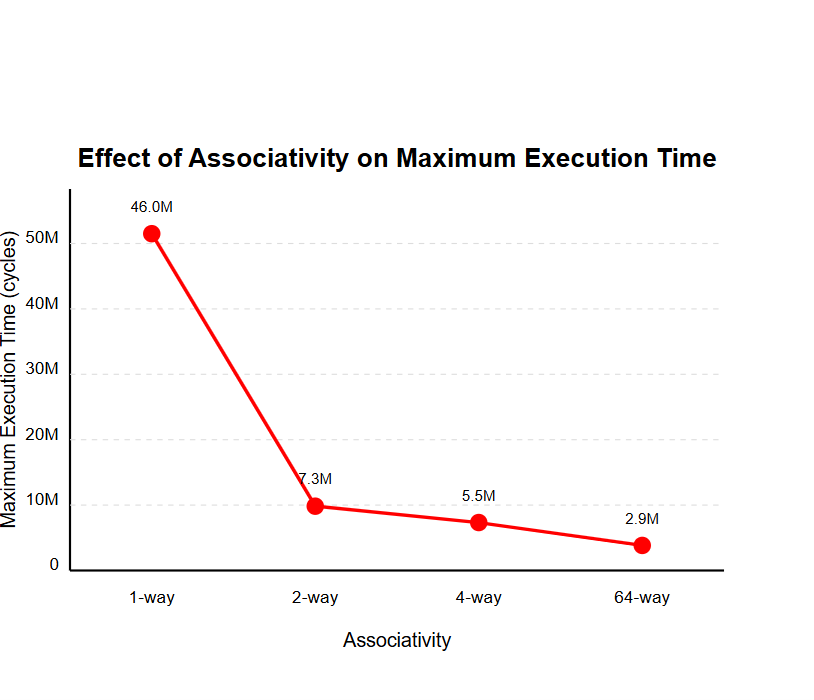
\includegraphics[width=0.8\textwidth]{image1_s3.png}
    \caption{Performance vs. Parameter}
    \label{fig:performance}
\end{figure}

\begin{figure}[H]
    \centering
    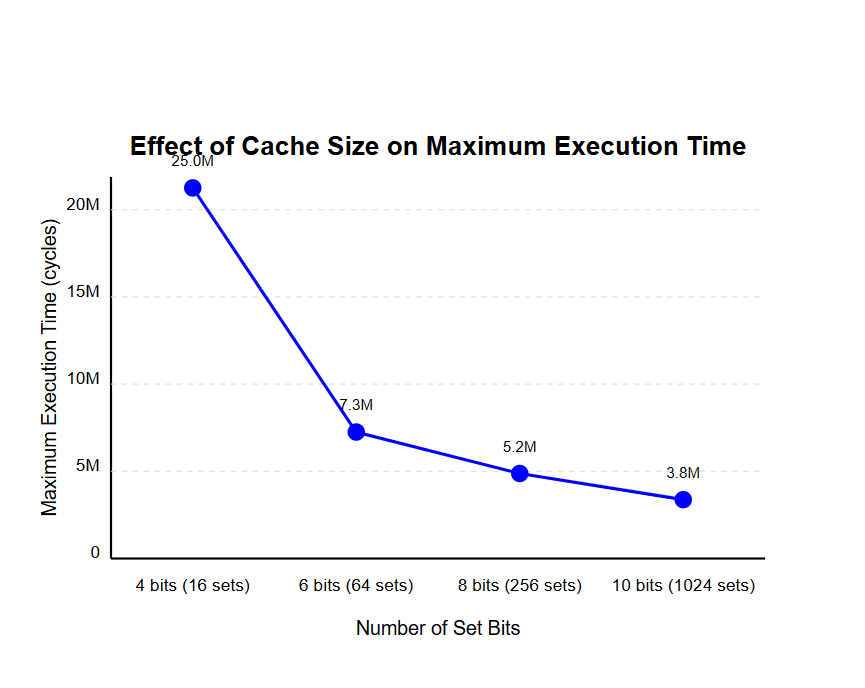
\includegraphics[width=0.8\textwidth]{image2_s3.png}
    \caption{Another performance metric}
    \label{fig:performance2}
\end{figure}

\begin{figure}[H]
    \centering
    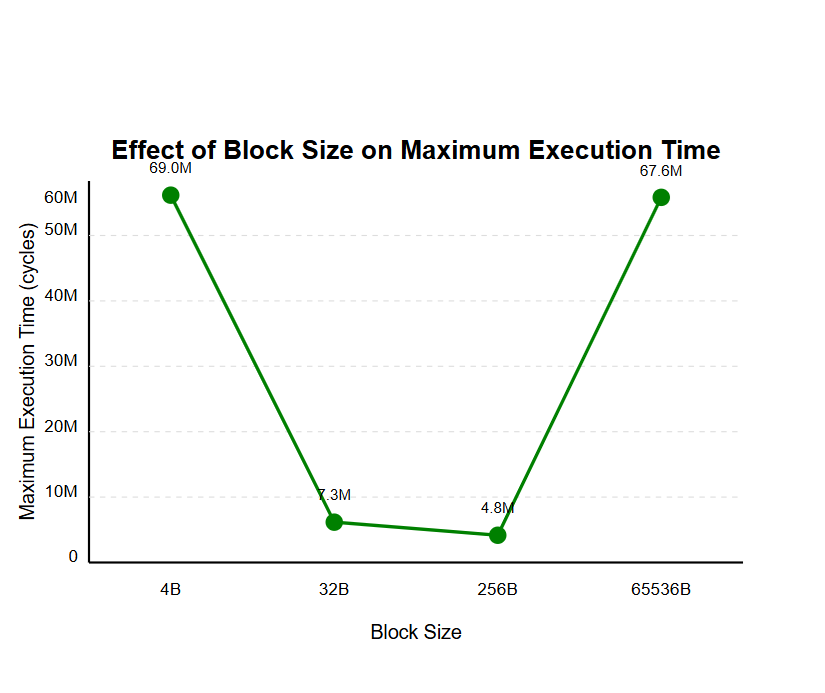
\includegraphics[width=0.8\textwidth]{image3_s3.png}
    \caption{Block size}
    \label{fig:block-size}
\end{figure}

\subsection{Effect of Cache Size (Number of Set Bits)}

\begin{figure}[H]
    \centering
    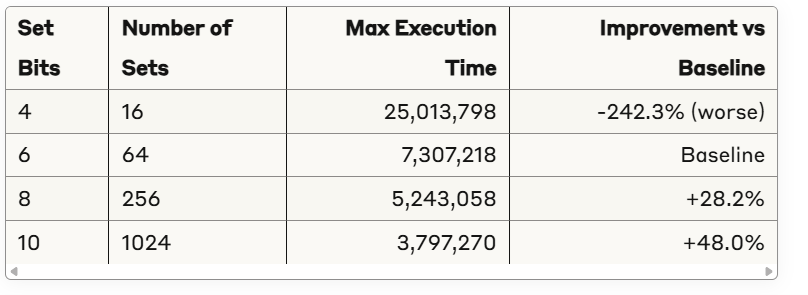
\includegraphics[width=0.8\textwidth]{image4_s3.png}
    \caption{Effect of Cache Size}
    \label{fig:cache-size}
\end{figure}

\subsubsection*{Analysis:}
\begin{itemize}
    \item Increasing the cache size has a significant positive impact on performance
    \item Going from 16 sets to 64 sets (4 to 6 bits) reduces execution time by 70.8\%
    \item Additional increases show diminishing returns, with 1024 sets providing only 48\% improvement over 64 sets
\end{itemize}

\textbf{Explanation:} Having a greater number of set bits decreases the execution time (up to the point recorded) because a greater number of blocks are stored in the cache at any time, decreasing the miss rate and thus avoiding the greater time taken to access from memory. There is a significant improvement from 4 to 6 set bits, because extremely low (4) bits in the cache lead to a very large portion of accesses being misses and frequent eviction of data.

\begin{figure}[H]
    \centering
    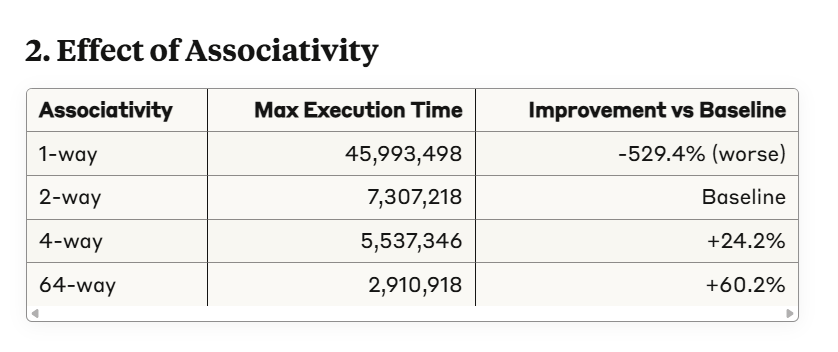
\includegraphics[width=0.8\textwidth]{image5_s3.png}
    \caption{Effect of Associativity}
    \label{fig:associativity}
\end{figure}

\subsubsection*{Analysis:}
\begin{itemize}
    \item Direct-mapped caches (1-way) perform very poorly due to conflict misses
    \item The jump from direct-mapped to 2-way associative yields a massive 84.1\% reduction in execution time
    \item Higher associativity continues to improve performance, with 64-way showing the best results
    \item This suggests the workload has significant conflict misses that benefit from higher associativity
\end{itemize}

\textbf{Explanation:} We find the associativity increase also keeps on decreasing execution time, although the decrease is very minimal at higher associativity. A greater associativity decreases the execution time by decreasing the number of evictions; a block occupying the same address (set bits in the cache) need not evict another block in the cache if it is occupied, and for a fully associative (64 size) set, a block can be placed anywhere in the cache, making the need for evictions very minimal.

\begin{figure}[H]
    \centering
    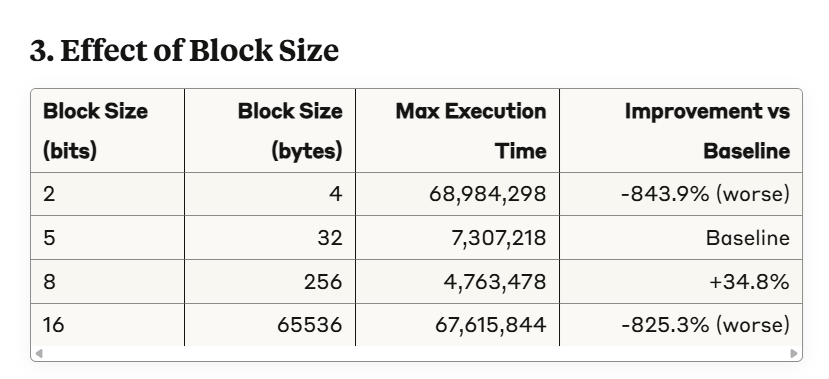
\includegraphics[width=0.8\textwidth]{image6_s3.png}
    \caption{Effect of Block Size}
    \label{fig:block-size-effect}
\end{figure}

\subsubsection*{Analysis:}
\begin{itemize}
    \item Block size shows a U-shaped curve in performance impact
    \item Very small blocks (4 bytes) perform extremely poorly
    \item Very large blocks (64KB) perform almost as poorly as very small blocks
    \item The optimal range appears to be between 32 bytes and 256 bytes
    \item Small blocks (4B) fail to exploit spatial locality, causing excessive misses
    \item Very large blocks (64KB) waste bandwidth and cause excessive evictions/conflicts
\end{itemize}

\textbf{Explanation:} A U shaped curve is expected when varying block size. Initially, increases in the block size are beneficial, as they utilise spatial locality more (a greater range of words around an accessed word are accessible when a block is brought into the cache) which means, as per spatial locality when nearby words are accessed there is lesser likelihood of misses. However, after a point increases lead to decrease in execution time because increasing block size also increases the miss penalty (when misses do occur, a larger number of bytes need to be transferred back into memory) and also increases competition for blocks (a greater block size means the cache can accommodate fewer blocks, leading to more misses).

\end{document}